\documentclass[
12pt,
 a4paper,
 % chapter=TITLE,
  % section=TITLE,
   % subsection=TITLE,
    % subsubsection=TITLE,
    english,
    brazil,
    % openright,
    % twoside
    oneside
    ]{abntex2}
    
% Pacotes
% ---
\usepackage[brazilian,hyperpageref]{backref}
\usepackage[alf]{abntex2cite}
\usepackage[utf8]{inputenc}
\usepackage[T1]{fontenc}
\usepackage{amsmath, amsfonts, amssymb}
\usepackage{float}
\usepackage{graphicx}
\usepackage{indentfirst}
\usepackage{hyperref}
\usepackage{geometry}
\usepackage{times}
\usepackage{setspace}
\usepackage{microtype}
\usepackage{color}
\usepackage{tikz} 
\usetikzlibrary{positioning,shapes.geometric}
% ---


% Configurações de margens
\geometry{
	a4paper,
	left=3cm,
	right=2cm,
	top=3cm,
	bottom=2cm
}

% Configurações do pacote backref
% Usado sem a opção hyperpageref de backref
\renewcommand{\backrefpagesname}{Citado na(s) página(s):~}
% Texto padrão antes do número das páginas
\renewcommand{\backref}{}
% Define os textos da citação
\renewcommand*{\backrefalt}[4]{
	\ifcase #1 %
	%
	\or
	Citado na página #2.%
	\else
	Citado #1 vezes nas páginas #2.%
	\fi}%
% ---

% Dados do TCC/Monografia
\titulo{Transformações Lineares e suas aplicações}
\autor{Hyslan Silva Cruz\\Iara Regina Grilo Papais\\Carolina Cristina Ferreira de Mello Pires}
\orientador[Orientadora:]{Lorena Salvi Stringheta}
\instituicao{Universidade Virtual do Estado de São Paulo} 
\local{Suzano}
\data{2024}
\tipotrabalho{TCC}
\preambulo{Monografia de graduação à Universidade Virtual do Estado de São Paulo, como requisito parcial para a obtenção do título de Licenciatura em Matemática.
	\\Orientadora: \imprimirorientador}


% Configurações de aparência do PDF final
% alterando o aspecto da cor azul
\definecolor{blue}{RGB}{41,5,195}

% informações do PDF
\makeatletter
\hypersetup{
	%pagebackref=true,
	pdftitle={\@title}, 
	pdfauthor={\@author},
	pdfsubject={\imprimirpreambulo},
	pdfcreator={LaTeX with abnTeX2},
	pdfkeywords={abnt}{latex}{abntex}{abntex2}{trabalho acadêmico}, 
	colorlinks=true,       		% false: boxed links; true: colored links
	linkcolor=black,          	% color of internal links
	citecolor=black,        		% color of links to bibliography
	filecolor=magenta,      		% color of file links
	urlcolor=blue,
	bookmarksdepth=4
}
\makeatother
% --- 

% ---
% Posiciona figuras e tabelas no topo da página quando adicionadas sozinhas
% em um página em branco. Ver https://github.com/abntex/abntex2/issues/170
\makeatletter
\setlength{\@fptop}{5pt} % Set distance from top of page to first float
\makeatother
% ---

% --- 
% Espaçamentos entre linhas e parágrafos 
% --- 

% O tamanho do parágrafo é dado por:
\setlength{\parindent}{1.3cm}

% Controle do espaçamento entre um parágrafo e outro:
\setlength{\parskip}{0.2cm}  % tente também \onelineskip

% Início do Documento
\begin{document}
	
	\selectlanguage{brazil}
	
	% Retira espaço extra obsoleto entre as frases.
	\frenchspacing 
	
	
	\renewcommand{\imprimircapa}{%
		\begin{capa}%
			\center
			{\ABNTEXchapterfont\large\imprimirautor}
			\vspace*{\fill}
			
			{\ABNTEXchapterfont\bfseries\LARGE\imprimirtitulo}
			
			\vspace*{5cm}
			\href{teste.com.br}{\textbf{Link do vídeo}}
			\vspace*{\fill}
			
			{\large\imprimirlocal}
			\par
			{\large\imprimirdata}
			\vspace*{1cm}
		\end{capa}
	}
	% Capa
	\imprimircapa
	% \href{teste.com.br}{video}
	
	% Folha de Rosto
	\imprimirfolhaderosto
	
	% ---
	% Dedicatória
	% ---
	\begin{dedicatoria}
		\vspace*{\fill}
		\centering
		\noindent
		\textit{
			Este trabalho é dedicado às crianças adultas que,\\
			quando pequenas, sonharam em se tornar cientistas.\\
			}
	\end{dedicatoria}
	% ---
	
	% ---
	% Agradecimentos
	% ---
	\begin{agradecimentos}
		A conclusão desta monografia representa um marco importante em nossas vidas acadêmica e profissional. Ao longo dessa jornada, tivemos a oportunidade de contar com o apoio e a colaboração de diversas pessoas e instituições, às quais expresso minha mais profunda gratidão.
		
		À minha família e amigos,
		
		minha base sólida e porto seguro em todos os momentos. Agradeço por acreditarem em nosso potencial, por incentivarem nossos sonhos e por celebrarem cada conquista ao nosso lado. A vocês, dedico este trabalho com imenso amor e reconhecimento.
		
		A  minha orientadora, Professora \imprimirorientador,
		
		reconheço a importância fundamental de sua orientação, sabedoria e paciência ao longo da pesquisa. Sua expertise e dedicação nos inspiraram e guiaram na construção deste trabalho. Agradeço pelas valiosas contribuições, pelo tempo dedicado e pela confiança depositada em nosso grupo.
		
		Aos demais membros da banca examinadora,
		
		Professores(as),
		
		agradeço a oportunidade de apresentar nossa pesquisa e receber seus valiosos feedbacks. Agradeço por terem dedicado seu tempo e conhecimento à avaliação deste trabalho.
		
		À \imprimirinstituicao,
		
		minha segunda casa durante os anos de graduação. Agradeço à instituição por nos proporcionar uma formação de qualidade, por nos colocar em contato com professores excepcionais e por nos oferecer os recursos necessários para o desenvolvimento desta pesquisa de forma gratuita.
		
		Aos colegas de curso e amigos da Licenciatura em Matemática,
		
		com quem compartilhamos momentos de aprendizado, desafios e alegrias. Agradeço pelas trocas de conhecimento, pelo apoio mútuo e pela amizade que nos acompanham desde o início da graduação.
		
		Aos projetos integradores e demais serviços de pesquisa além da plataforma acadêmica,
		
		que nos proporcionaram acesso a materiais essenciais para a realização deste trabalho. Agradeço a todos os profissionais que me auxiliaram na busca por informações e na utilização de ferramentas para uma boa pesquisa.
		
		A todos que, direta ou indiretamente, contribuíram para a realização deste trabalho,
		
		nossa sincera gratidão. Cada palavra de incentivo, cada sugestão e cada ajuda foram valiosas para o nosso aprimoramento e para a conquista deste objetivo.
		
		Este trabalho é fruto de um esforço coletivo e representa a soma de conhecimentos, experiências e apoio de muitas pessoas. Agradecemos a todos que fizeram parte dessa jornada e que nos ajudaram a alcançar este importante marco em nossas vidas.
	\end{agradecimentos}
	% ---
	
	% ---
	% Epígrafe
	% ---
	\begin{epigrafe}
		\vspace*{\fill}
		\begin{flushright}
			\textit{``Hoje, ainda almejamos saber por que\\
				estamos aqui e de onde viemos.O desejo\\
				profundo da humanidade pelo	conhecimento é\\
				justificativa suficiente para nossa busca contínua.\\
				(Stephen Hawking)}
		\end{flushright}
	\end{epigrafe}
	% ---
	
	
	% Resumo
	% resumo em português
	\setlength{\absparsep}{18pt} % ajusta o espaçamento dos parágrafos do resumo
	\begin{resumo}
		Só após ao fim da conclusão.
		
		\textbf{Palavras-chave: Transformação Linear, Álgebra Linear, Matrizes}
	\end{resumo}
		
	
	% Abstract
	% resumo em inglês
	\begin{resumo}[Abstract]
		\begin{otherlanguage*}{english}
			Same above.
			
			\vspace{\onelineskip}
			
			\noindent 
			\textbf{Keywords}: Linear Transformation, Linear Algebra. Matrices.
		\end{otherlanguage*}
	\end{resumo}
	
	% inserir lista de tabelas
	% ---
	\pdfbookmark[0]{\listtablename}{lot}
	\listoftables*
	\cleardoublepage
	% ---
	
	% Lista de símbolos
	\begin{simbolos}
		\item[$ \mathbb{R} $] Conjunto dos números reais.
		\item[$\exists$] Existe.
		\item[$\in$] Pertence.
		\item[$\mid$] Tal que.
		\item[$\therefore$] Portanto.
		\item[$\emptyset$] Conjunto vazio.
		\item[$\sigma$] Somatório.
	\end{simbolos}
	
	
	% Sumário
	\pdfbookmark[0]{\contentsname}{toc}
	\tableofcontents*
	\cleardoublepage
	
	
	% Capítulos
	\textual
	
	\chapter{Introdução}
Uma área da Matemática que tem implicações na computação gráfica, genética, criptografica, redes elétricase outros é a Álgebra Linear (AL). Com estrutura que permite um tratamento algébrico simples, a AL estuda os aspectos relacionados ao Espaço Vetorial (EV). Um conceito central da AL é a Transformação Linear (TL), que desempenham papel fundamental na análise e compreensão dos sistemas lineares de equações, geometria analítica, física, engenharia e outros campos de estudo. % Citar Rios,Figueiredo e Cunha, 2009

Contextualizando o início dos estudos da AL, que é o estudo dos espaços vetoriais e das TL entre eles e possui variadas aplicações % citar Souza SIlva e Costa da SIlva, 2017
, nos meados do século XVIII, Euler e Louis Lagrange publicaram o "Recherche d'Arithmétique", entre 1773 e 1775, no qual estudavam certos conceitos da TL. Posteriormente, Johann Carl Friedrich Gauss, também estudou sobre assuntos que apresentou similaridade com a matriz de transformação linear.

No século XIX e XX, Giuseppe Peano cunha o termo "sistema linear" com a primeira definição de axiomática para espaço vetorial. Nos dias atuais, a apresentação da AL, temas abordados nesse campo da matemática são frequentemente esquecidos. Este estudo busca o entendimento e compreender sobre as transformações lineares em sua totalidade e aplicações no contexto atual contemporâneo.

Passo esse brevíssimo contexto histório e motivador para a nossa pesquisa e deleite desramo de estudado, iremos nos adiantar a certos conceitos matemáticos elementares já bastantes fundamentados no decorrer dos anos escolares do ensino básico regular. para isto, passaremos a certas definições matemáticas primordiais que serão apresentadas nesta monografia para as discussões advindas a posteriori neste estudo.

Portanto, divimos esta monografia em 4 capítulos: revisão literária fundamentais, pesquisas de artigos, teses e discussões recentes sobre as transformações lineares em diversas aplicações, seu contexto educacional atual em questão de matéria aplicada e por conseguinte...

		
	\chapter{Espaços Vetoriais}
Começaremos pela definição de um espaço vetorial utilizando aquelas apresentadas por \cite{boldrini1980} e \cite{ulhoa2018}, onde, podemos tratar como um vetor ao designar um elemento do espaço vetorial de um número $\mathbb{R}$ definido tal que:

\noindent\textbf{Definição 01:} Seja um conjunto V, não vazio, com duas operações: soma, $(v_1, v_2) \rightarrow v_1 + v_2$, e multiplicação por escalar, $(k, v) \rightarrow kv$, tais que, para quaisquer $u, v, w \in \mathbf{V}$ e $a, b \in \mathbb{R}$, satisfaçam as propriedades: \nocite{boldrini1980}

\begin{enumerate}
	\item $1u = u$.
	\item $\exists$ $0$ $\in V$ tal que $u + 0 = u$.
	\item $\exists$ $-u \in V$ tal que $u + (-u) = 0$.
	\item $a(u + v) = au + av$.
	\item $(a + b)v = av + bv$.
	\item $(ab)v = a(bv)$.
\end{enumerate}

\noindent\textbf{Observação:} $\textbf{0}$ é o vetor nulo. \nocite{ulhoa2018}

\noindent\textbf{Observação:} Limitaremos nossa discussão, demonstrações e aplicações dentro do conjunto dos números reais apenas.

\noindent\textbf{Exemplo 01:} Suponhamos dois pontos no plano, o ponto $\mathbf{O}_{(0, 0)}$ sendo a origem e $\mathbf{M}_{(2, 2)}$, onde, se $\vb{V}$, é um conjunto não vazio e possui a soma desses dois pontos ($\mathbf{O}_{(0, 0)}$ e $\mathbf{M}_{(2, 2)}$). Além disso, seu escalar pertencente ao conjunto dos $\mathbb{R}$, que satisfazem todas as propriedades de um espaço vetorial. Logo $\vb{V}$ é um espaço vetorial.

\begin{figure}[H]
	\centering
	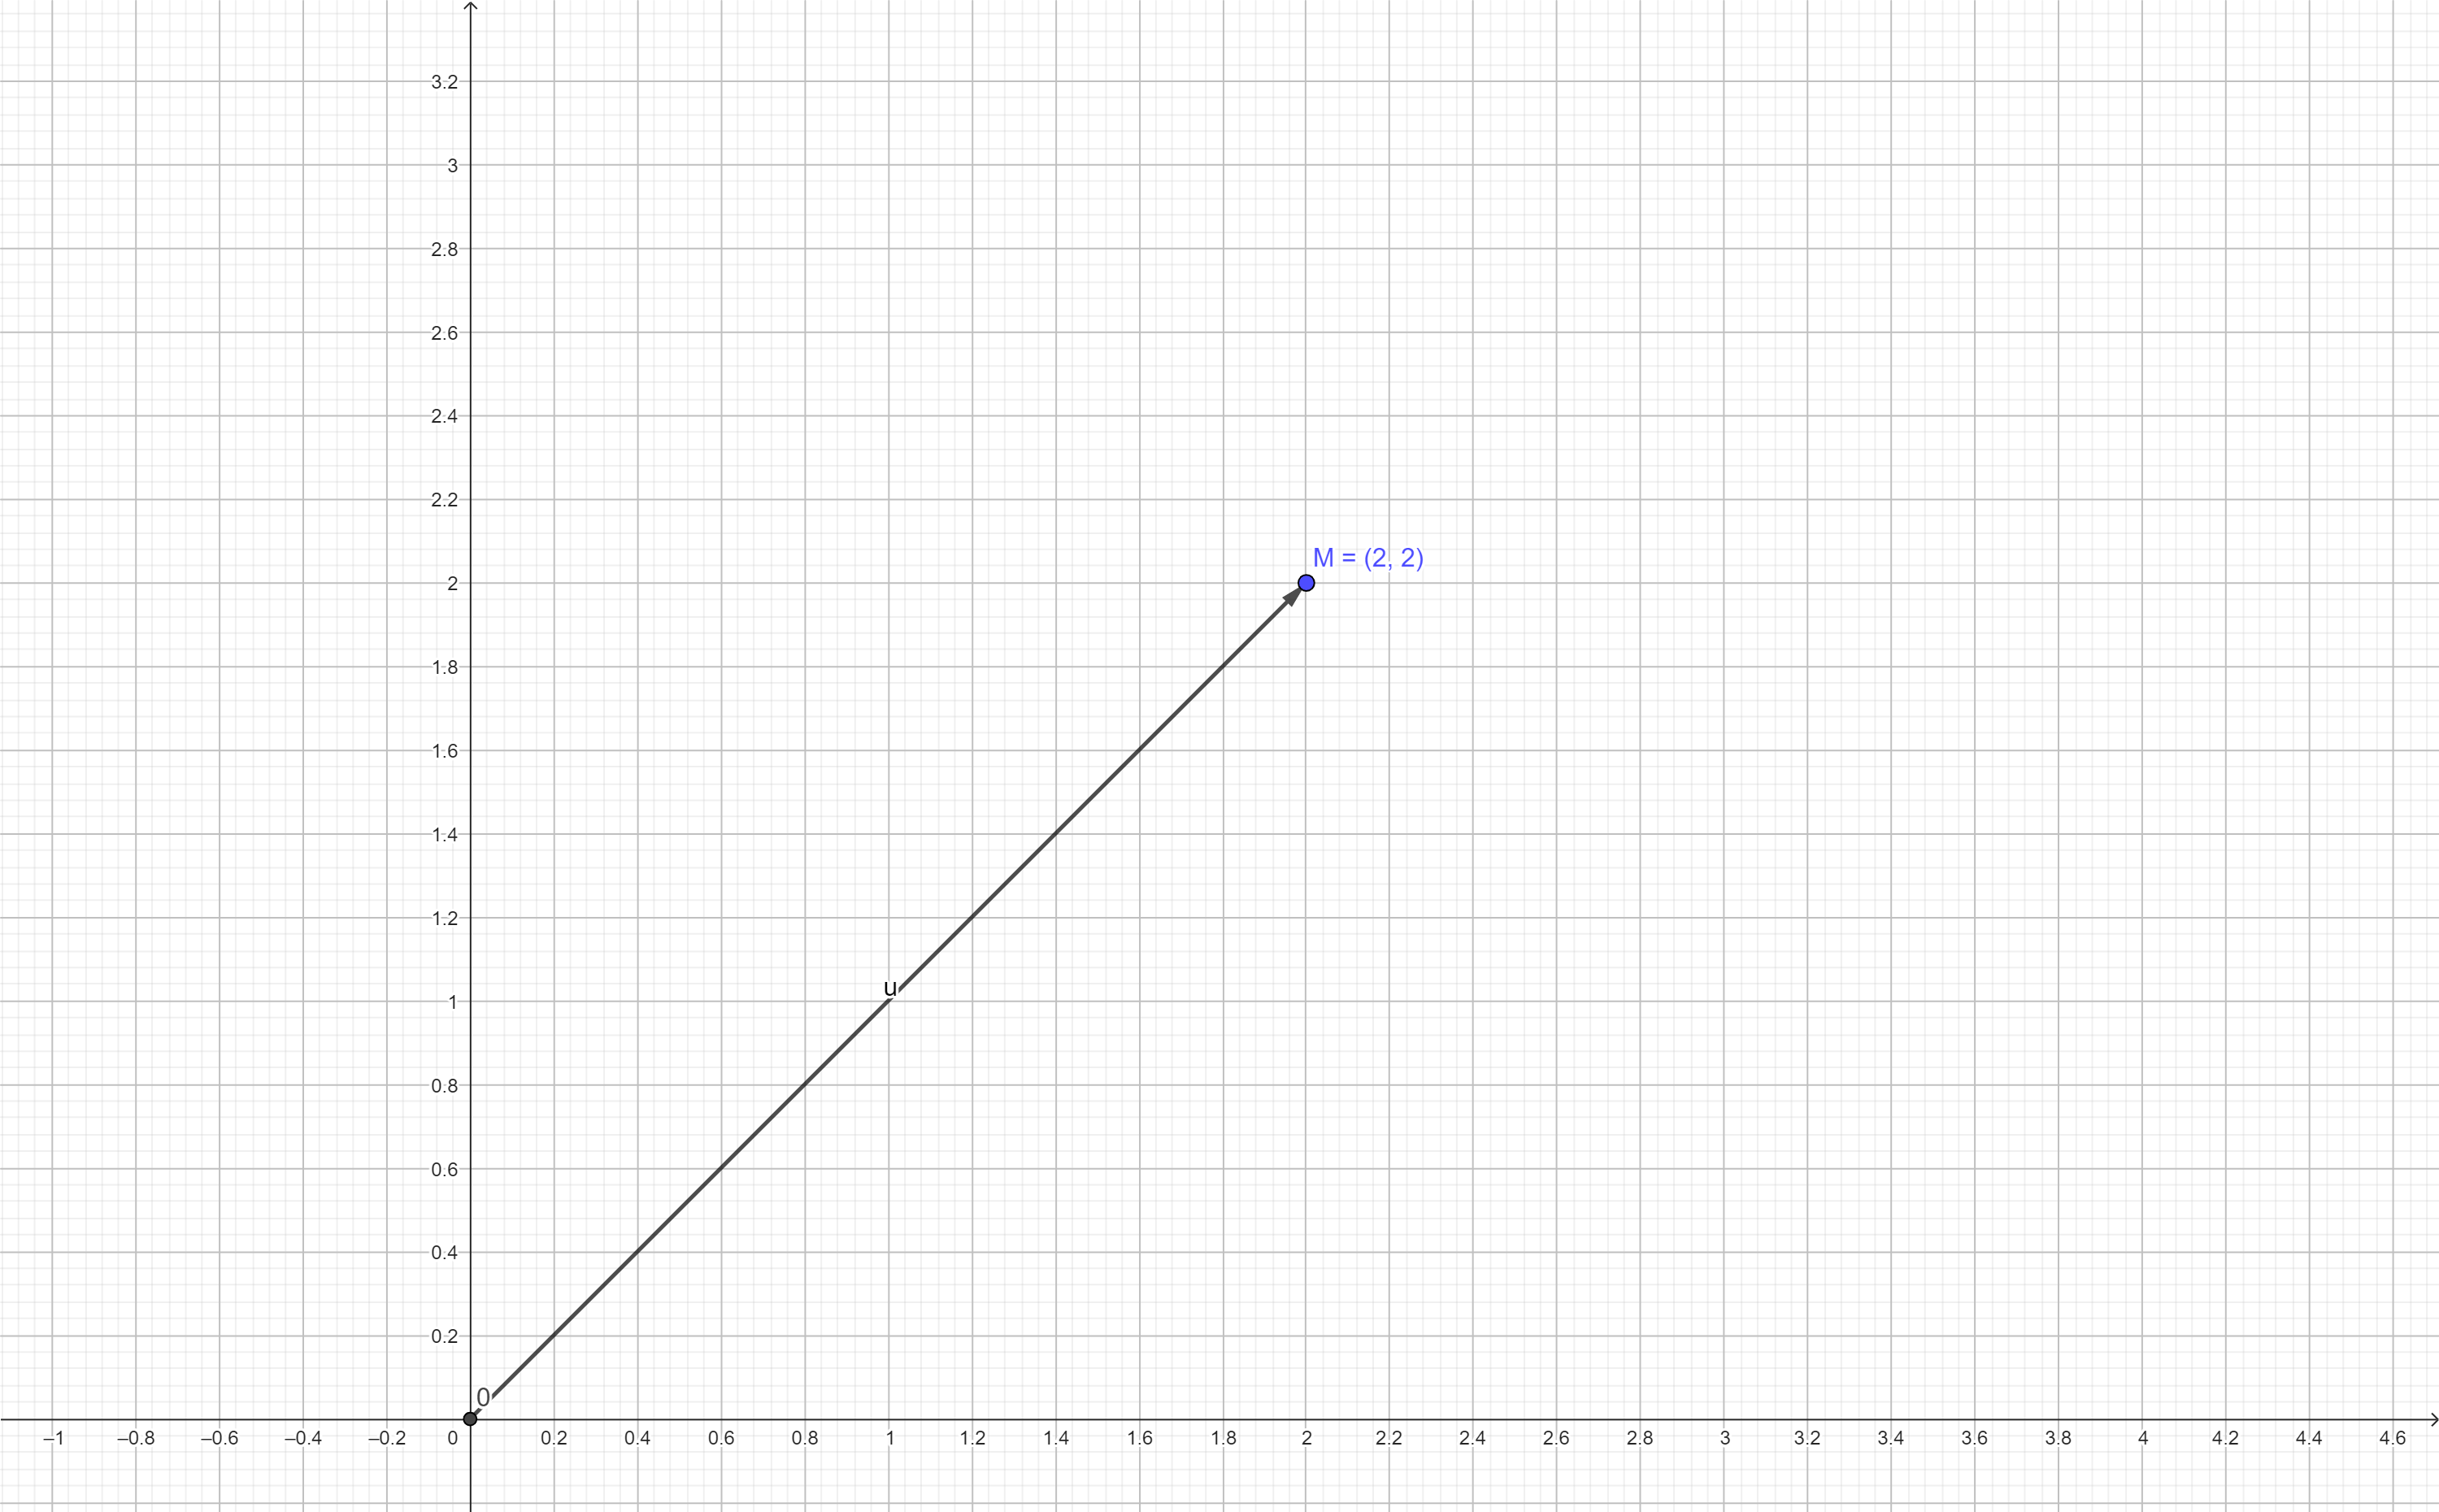
\includegraphics[scale=2.00]{exemplo01.png}
	\caption{Um vetor no plano.}
\end{figure}

A partir disto, podemos perceber o uso analítico dos espaços vetoriais para resolução de problemas em geral. Vejamos mais alguns exemplos.

\noindent\textbf{Exemplo 02:} O exemplo anterior, trata-se de uma matriz de $\mathbb{R}^2$ pode ser dito como, no plano, agora iremos expandir para $\mathbb{R}^3$, seja um vetor $A = (x, y, z)$ ou representado pela forma matricial:

\[
A = \begin{bmatrix}
	a \\ b \\ c
\end{bmatrix}
\]
\noindent Assim, por quaisquer números reais, podemos fazer uma projeção ortogonal no espaço, segue um exemplo traçado:

\begin{figure}[H]
	\centering
	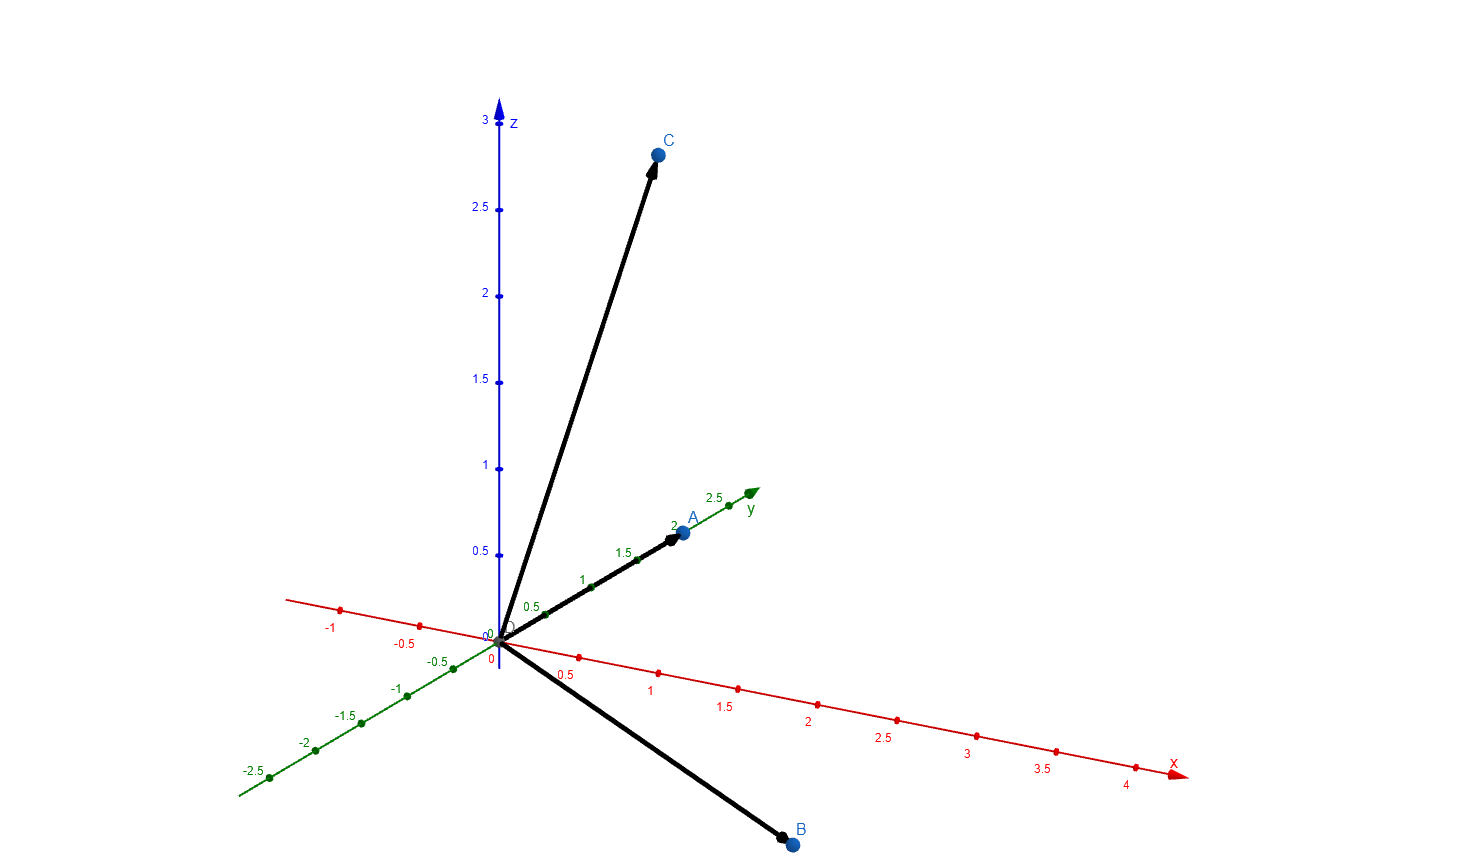
\includegraphics[scale=0.30]{exemplo02.png}
	\caption{Exemplo de vetor no espaço.}
\end{figure}

\noindent\textbf{Exemplo 03:} Consideremos $n-uplas$ de números reais.

\begin{equation}
	V = \mathbb{R}^n = \{(x_1, x_2, \ldots, x_n); x_i \in \mathbb{R}\}
\end{equation}

\noindent e se \( u = (x_1, x_2, \ldots, x_n) \), \( v = (y_1, y_2, \ldots, y_n) \) e \( a \in \mathbb{R} \),

\[
u + v = (x_1 + y_1, x_2 + y_2, \ldots, x_n + y_n) \quad \text{e} \quad a u = (ax_1, ax_2, \ldots, ax_n)
\]


Por tratarmos de uma quantidade $n$ de números, o campo tridimensional deixa de ser visto, e passamos a ter $\mathbb{R}^n$ dimensões, as propriedades não deixam de valer independente a quantidade de dimensões.

\section{Subespaços Vetoriais}
Nesta seção iremos introduzir conceitos no estudo de espaço vetorial para subespaço vetorial.

\noindent\textbf{Definição 02:} Dado um espaço vetorial V, um subconjunto W, não vazio, será um subespaço vetorial de V se:
\begin{enumerate}
	\item Para quaisquer $u, v \in W$ tivermos $u + v \in W$.
	\item Para quaisquer $a \in R, u \in W$ tivermos $au \in W$.
	\end{enumerate}

\noindent\textbf{Teorema 01:} Um subconjunto não vazio $W$ de $V$ é um subespaço de $V$ se, e somente se, para cada par de vetores $\alpha, \beta$ em $W$ e cada escalar $c$ em $F$, o vetor $c\alpha + \beta$ está em $W$.

\noindent\textbf{Demonstração:} Suponhamos que $W$ seja um subconjunto não vazio de $V$, tal que, $c\alpha + \beta$ pertença a $W$ para todos os vetores $\alpha$, $\beta$ em $W$ e todos escalares $c$ em $F$. Como $W$ é não vazio, existe um vetor $\rho$ em $W$, logo $(-1) \rho + \rho = 0$ está em $W$. Então se $\alpha$ é um vetor arbitrário em $W$ e $c$ é um escalar arbitrário, o vetor $c\alpha = c\alpha + 0$ está em $W$. Em particular $(-l)\alpha = -\alpha$ está em $W$. Finalmente se $\alpha$ e $\beta$ estão em $W$, então $\alpha + \beta = 1\alpha + \beta$ está em $W$.
Assim, $W$ é um subespaço de $V$. \nocite{hoffman1979}

\noindent\textbf{Exemplo 04:} Considere o espaço vetorial $\mathbb{R}^3$. O conjunto de todos os vetores que residem no plano $xy$, ou seja, $\{(x, y, 0) \mid x, y \in \mathbb{R}\}$, forma um subespaço vetorial de $\mathbb{R}^3$.

Se o conjunto dado forma um subespaço vetorial de $\mathbb{R}^3$, precisamos verificar as três propriedades fundamentais:

\begin{enumerate}
    \item Contém o vetor nulo: O vetor nulo em $\mathbb{R}^3$ é $(0,0,0)$. Este vetor também está contido no plano $xy$, pois $z = 0$.
    
    \item É fechado sob adição: Se tomarmos dois vetores $(x_1, y_1, 0)$ e $(x_2, y_2, 0)$ no plano $xy$, a sua soma será $(x_1 + x_2, y_1 + y_2, 0)$, que também reside no plano $xy$.
    
    \item É fechado sob multiplicação por escalar: Para qualquer escalar $c$ e vetor $(x, y, 0)$ no plano $xy$, $c \cdot (x, y, 0) = (cx, cy, 0)$, que também está no plano $xy$.
\end{enumerate}

Então, o conjunto de todos os vetores $(x, y, 0)$ com $x, y \in \mathbb{R}$ forma um subespaço vetorial de $\mathbb{R}^3$.

\noindent\textbf{Exemplo 05:} No espaço vetorial das funções reais de uma variável real, $V = \{f(x) \mid f: \mathbb{R} \rightarrow \mathbb{R}\}$, considere o conjunto de todas as funções lineares, ou seja, $\{f(x) = mx + b \mid m, b \in \mathbb{R}\}$. Esse conjunto forma um subespaço vetorial de $V$. Novamente, você pode verificar as propriedades para confirmar.

Se o conjunto dado forma um subespaço vetorial de $V$, novamente precisamos verificar as três propriedades fundamentais:

\begin{enumerate}
    \item Contém a função nula: A função nula em $V$ é $f(x) = 0$. Esta função é uma função linear, pois pode ser escrita como $f(x) = 0 \cdot x + 0$. Portanto, a função nula está contida no conjunto.
    
    \item É fechado sob adição: Se tomarmos duas funções lineares $f_1(x) = m_1x + b_1$ e $f_2(x) = m_2x + b_2$, a sua soma será $f_1(x) + f_2(x) = (m_1 + m_2)x + (b_1 + b_2)$, que também é uma função linear. Portanto, o conjunto é fechado sob adição.
    
    \item É fechado sob multiplicação por escalar: Para qualquer escalar $c$ e função linear $f(x) = mx + b$, a multiplicação por escalar $cf(x) = c(mx + b) = (cm)x + (cb)$ também é uma função linear. Assim, o conjunto é fechado sob multiplicação por escalar.
\end{enumerate}

Portanto, o conjunto de todas as funções lineares $f(x) = mx + b$ com $m, b \in \mathbb{R}$ forma um subespaço vetorial de $V$.

\noindent\textbf{Exemplo 06:} No espaço das matrizes reais $2 \times 2$, $M_{(2,2)}$, considere o conjunto de todas as matrizes simétricas, ou seja, aquelas em que $A = A^T$. Esse conjunto forma um subespaço vetorial de $M_{(2,2)}$. Você pode demonstrar isso verificando as propriedades de um subespaço vetorial

Para tal, é imperativo investigar as três propriedades basilares:

\begin{enumerate}
    \item \textbf{Presença da Matriz Nula:} A matriz nula em $M_{(2,2)}$ é a matriz $\begin{pmatrix} 0 & 0 \\ 0 & 0 \end{pmatrix}$. Nota-se que esta matriz é simétrica, posto que $A = A^T$. Portanto, a matriz nula está asseguradamente contida no conjunto em questão.
    
    \item \textbf{Fechamento sob Adição:} Considerando duas matrizes simétricas $A$ e $B$, a sua soma $A + B$ é também simétrica, visto que $(A + B)^T = A^T + B^T = A + B$. Logo, o conjunto demonstra ser fechado sob adição.
    
    \item \textbf{Fechamento sob Multiplicação por Escalar:} Para qualquer escalar $c$ e matriz simétrica $A$, a multiplicação por escalar $cA$ é igualmente simétrica, haja vista que $(cA)^T = cA^T = cA$. Deste modo, o conjunto revela-se fechado sob multiplicação por escalar.
\end{enumerate}

Assim sendo, constata-se que o conjunto de todas as matrizes simétricas configura-se como um subespaço vetorial de $M_{(2,2)}$.

\section{Combinação Linear}
Dentro de um espaço vetorial, conforme demonstrado que podemos ter subconjuntos de espaços vetoriais, é possível a obtenção de novos vetores a partir de vetores dados \cite{boldrini1980}.

\noindent\textbf{Definição 03:} Sejam $V$ um espaço vetorial, $v_1, v_2, \ldots, v_n \in V$ e $a_1, \ldots, a_n \in \mathbb{R}$. Então, o vetor $v = a_1v_1 + a_2v_2 + \ldots + a_nv_n$ é um elemento de $V$ podendo ser chamado combinação linear de $v_1, \ldots, v_n$.


Seja \( V \) um subespaço de \( W \) (\( V \subset W \)). Se \( W \) é gerado pelos vetores \( v_1, \ldots, v_n \), podemos adotar a notação \( W = [v_1, \ldots, v_n] \). Isso significa que \( W \) é o conjunto de todas as combinações lineares dos vetores \( v_1, \ldots, v_n \). A notação expandida é:

\begin{equation}
	W = [v_1, \ldots, v_n] = \left\{ v \in W \;\middle|\; v = a_1v_1 + \ldots + a_nv_n, \; a_i \in \mathbb{R}, \; 1 \leq i \leq n \right\}
\end{equation}


\noindent\textbf{Exemplo 07:} Presuma um vetor $V = \mathbb{R}^3, v \in V, v \neq 0$. Se imaginarmos sua reta que contém o vetor $v$, onde, $[v] = {av: a \in \mathbb{R}}$

\begin{figure}[H]
	\centering
	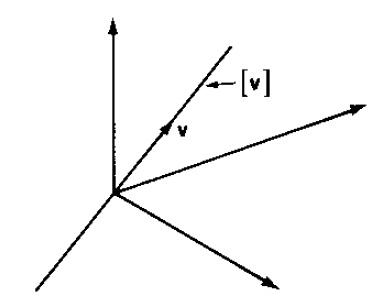
\includegraphics[scale=0.90]{cb_exemplo7.png}
	\caption{Combinação linear de Vetores \cite{boldrini1980}, pg. 113.}
\end{figure}

\noindent\textbf{Exemplo 08:} Se obtemos $v_1, v_2 \in \mathbb{R}^3$ e $v_3 \in [v_1, v_2]$, então $[v_1, v_2, v_3] = [v_1, v_2]$, então $v_3$ é um combinação linear de  $v_1$ e $v_2$.

\begin{figure}[H]
	\centering
	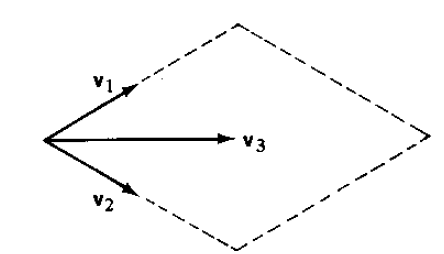
\includegraphics[scale=0.90]{cb_exemplo8.png}
	\caption{Combinação de três vetores lineares \cite{boldrini1980}, pg. 113.}
\end{figure}

\noindent\textbf{Exemplo 09:} Consideremos o espaço vetorial $\mathbb{R}^3$ e os vetores $\mathbf{v} = \begin{pmatrix} 2 \\ 3 \\ 1 \end{pmatrix}$ e $\mathbf{w} = \begin{pmatrix} 1 \\ -1 \\ 2 \end{pmatrix}$. Sejam também os escalares $a = 3$ e $b = -1$. Então temos, os seguintes elementos.

\begin{table}[h]
	\centering
	\begin{tabular}{@{}ccc@{}}
		\toprule
		\textbf{Vetor} & \textbf{Componentes} & \textbf{Escalar} \\ \midrule
		$\mathbf{v}$   & $ 2, 3, 1$   & $3$              \\
		$\mathbf{w}$   & $ 1, -1, 2$  & $-1$             \\ \bottomrule
	\end{tabular}
	\caption{Vetores e escalares utilizados na combinação linear}
\end{table}

Definimos a combinação linear dos vetores $\mathbf{v}$ e $\mathbf{w}$ como:

\begin{equation}
	a\mathbf{v} + b\mathbf{w} = 3 \begin{pmatrix} 2 \\ 3 \\ 1 \end{pmatrix} + (-1) \begin{pmatrix} 1 \\ -1 \\ 2 \end{pmatrix}.
\end{equation}

Aplicando as operações, obtemos:

\begin{equation}
	a\mathbf{v} + b\mathbf{w} = \begin{pmatrix} 6 \\ 9 \\ 3 \end{pmatrix} + \begin{pmatrix} -1 \\ 1 \\ -2 \end{pmatrix} = \begin{pmatrix} 6 - 1 \\ 9 + 1 \\ 3 - 2 \end{pmatrix} = \begin{pmatrix} 5 \\ 10 \\ 1 \end{pmatrix}.
\end{equation}

Portanto, a combinação linear dos vetores $\mathbf{v}$ e $\mathbf{w}$ com os coeficientes $a = 3$ e $b = -1$ é o vetor 

\[
\begin{pmatrix} 5 \\ 10 \\ 1 \end{pmatrix}
\]


\section{Dependência e Independência Linear}
Dado a combinação linear, devemos saber, a priori, se algum desses vetores não é combinação linear dos outros e assim por diante. Para isto precisamos saber sua dependência e independência linear.\nocite{camargo2005}

\noindent\textbf{Definição 03:} Sejam $\mathbf{V}$ um espaço vetorial e $\mathbf{v}_1, \ldots, \mathbf{v}_n \in \mathbf{V}$. Dizemos que o conjunto ${\mathbf{v}_1, \ldots, \mathbf{v}_n}$ é linearmente independente (\textbf{LI}), ou que os vetores $\mathbf{v}_1, \ldots, \mathbf{v}_n$ são \textbf{LI}, se a equação

\begin{equation}
	a_1\mathbf{v}_1 + \ldots + a_n\mathbf{v}_n = 0
\end{equation}

\noindent implica que $a_1 = a_2 = \ldots = a_n = 0$. No caso em que exista algum $a_i \neq 0$ dizemos que ${v_1, \ldots, v_n}$ é linearmente dependente (\textbf{LD}), ou que os vetores $\mathbf{v}_1, \ldots, \mathbf{v}_n$ são \textbf{LD}.

\noindent\textbf{Teorema 02:} Um conjunto de vetores é linearmente dependente (\textbf{LD}) se, e somente se, pelo menos um dos vetores pode ser escrito como uma combinação linear dos outros. Logo,

\begin{equation}
\{\mathbf{v}_1, \ldots, \mathbf{v}_n \} \text{ é \textbf{LD}} \iff \exists i \in \{1, \ldots, n\} \text{ tal que } \mathbf{v}_i = \sum_{j \neq i} c_j \mathbf{v}_j \text{ para alguns } c_j \in \mathbb{R}
\end{equation}

\noindent\textbf{Demonstração:} Sejam $\mathbf{v}_1, \ldots, \mathbf{v}_n$ \textbf{LD} e $a_1\mathbf{v}_1 + \ldots + a_j\mathbf{v}_j + \ldots + a_n\mathbf{v}_n = 0$

\noindent Um dos coeficientes deve ser diferente de zero. Suponhamos que seja $a_j \neq 0$. Então 

\begin{equation}
	\mathbf{v}_j = -\frac{1}{a_j}(a_1\mathbf{v}_1 + \ldots + a_{j - 1}\mathbf{v}_{j - 1} + a_{j + 1}\mathbf{v}_{j + 1} + \ldots + a_n\mathbf{v}_n)
\end{equation}

\noindent e portanto $\mathbf{v}_j = -\frac{a_1}{a_j}\mathbf{v}_1 + \ldots -\frac{a_n}{a_j}\mathbf{v}_n$

\noindent Logo, $\mathbf{v}_j$ é uma combinação linear dos outros vetores.

\noindent\textbf{Exemplo 10:} Sejam $\mathbf{V} = \mathbb{R}^3$ e $v_1, v_2 \in \mathbf{V}$, $\{\mathbf{v}_1, \mathbf{v}_2\}$ é \textbf{LD} $\iff \mathbf{v}_1$ e $\mathbf{v}_2$ estiverem na mesma reta, que passa pela origem. $(\mathbf{v}_1 = \lambda\mathbf{v}_2)$.

\begin{figure}[H]
	\centering
	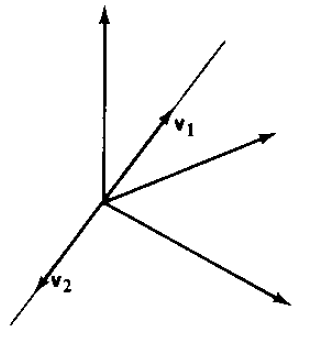
\includegraphics[scale=0.90]{cb_exemplo10.png}
	\caption{Vetores linearmente dependentes \cite{boldrini1980}, pg. 115.}
\end{figure}

\section{Base}
Seja $\mathbf{V}$ um espaço vetorial. Uma base para $\mathbf{V}$ é um conjunto finito $B = \{\mathbf{u}_1, \ldots, \mathbf{u}_n\}$ de elementos de $\mathbf{V}$ tal que $B$ é linearmente independente e gera o espaço vetorial $\mathbf{V}$, ou seja, qualquer elemento de $\mathbf{V}$ pode ser escrito como combinação linear dos elementos de $B$. Se o subespaço gerado por $B$ coincide com um subespaço $\mathbf{H}$ de um espaço vetorial $\mathbf{V}$, então

\begin{equation}
\mathbf{H} = \text{Span}\{\mathbf{b}_1, \ldots, \mathbf{b}_p\}
\end{equation}

A definição de base se aplica ao caso em $\mathbf{H} = \mathbf{V}$, porque todo espaço vetorial é subespaço dele mesmo. Assim, uma base de $\mathbf{V}$ é um conjunto linearmente independente que gera $\mathbf{V}$ \cite{lay1999}. Então se tivermos uma tripla ordenada linearmente independente $\mathbf{E} = (\va*{e}_1, \va*{e}_2, \va*{e}_3)$ será uma base de $\mathbf{V}^3$.

\begin{figure}[H]
	\centering
	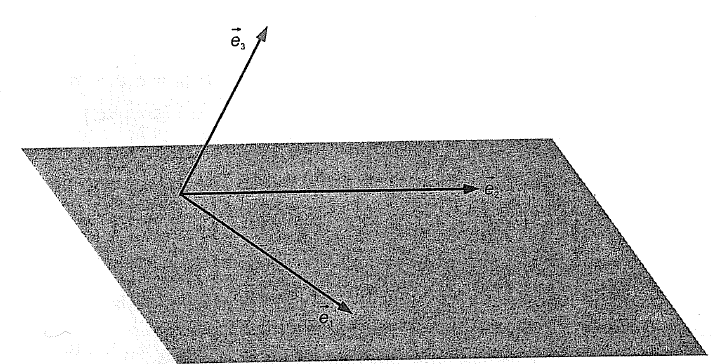
\includegraphics[scale=0.90]{b_v3.png}
	\caption{Base de um vetor em $\mathbb{R}^3$ \cite{camargo2005}, pg. 52.}
\end{figure}

Para analisar as propriedades da base de um espaço vetorial de forma generalizada, consideremos desta forma.

\noindent\textbf{Teorema 3:} Sejam $\mathbf{v}_1, \mathbf{v}_2, \ldots, \mathbf{v}_n \mid \mathbf{v} \neq 0$, estes que geram um espaço vetorial $\mathbf{V}$. Então, dentre este vetores podemos extrair uma base de $\mathbf{V}$.

Se $\mathbf{v}_1, \mathbf{v}_2, \ldots, \mathbf{v}_n$ são \textbf{LI}, então eles cumprem as condições para uma base, e não temos mais nada a fazer. Se $\mathbf{v}_1, \mathbf{v}_2, \ldots, \mathbf{v}_n$ são \textbf{LD}, então existe uma combinação linear deles, com algum coeficiente não zero, obtendo o vetor nulo

\begin{equation}
\mathbf{x}_1\mathbf{v}_1 + \mathbf{x}_2\mathbf{v}_2 + \ldots + \mathbf{x}_n\mathbf{v}_n = 0
\end{equation}

Se $\mathbf{x}_n \neq 0$. Então é possível escrever

\begin{equation}
\mathbf{v}_n = \frac{-\mathbf{x}_1}{\mathbf{x}_n}\mathbf{v}_1 + \frac{-\mathbf{x}_2}{\mathbf{x}_n}\mathbf{v}_2 + \ldots + \frac{-\mathbf{x}_{n -1}}{\mathbf{x}_n}\mathbf{v}_{n -1}
\end{equation}

ora, $\mathbf{v}_n$ é uma combinação linear de $\mathbf{v}_1, \ldots, \mathbf{v}_{n -1}$ e, portanto, $\mathbf{v}_1, \ldots, \mathbf{v}_{n -1}$ geram $\mathbf{V}$. Se $\mathbf{v}_1, \ldots, \mathbf{v}_{n -1}$ for \textbf{LD}, então existe uma combinação linear deles que dará o vetor nulo e com algum coeficiente $\neq 0$, portanto, é possível extrair o vetor que corresponde a este coeficiente. Se continuarmos, com as iterações, após uma quantidade $n$ de passos, obteremos um subconjunto de $\{\mathbf{v}_1, \ldots, \mathbf{v}_n\}$ formado por $r(r \leqslant n)$ vetores \textbf{LI} $\mathbf{v}_{i1}, \mathbf{v}_{i2}, \ldots, \mathbf{v}_{ir}$, que ainda geram $\mathbf{V}$, por fim, formará uma base.

\section{Dimensão}
A dimensão de um espaço vetorial $\mathbf{V}$ é o número de elementos de uma base para $V$, que denotamos por $\dim(\mathbf{V})$. Caso $\mathbf{V} = \{e\}$, o conjunto vazio é uma base para $V$ e $\dim(\mathbf{V}) = 0$. Qualquer base de um espaço vetorial tem sempre o mesmo número de elementos.

\noindent\textbf{Teorema 4:} Seja  $\mathbf{V}$ um espaço vetorial e $\{\mathbf{u}_1, \ldots, \mathbf{u}_n\}$ um conjunto de elementos que geram  $\mathbf{V}$. Então, dentre esses elementos podemos extrair uma base para $\mathbf{V}$.

\noindent\textbf{Teorema 5:} Seja $\mathbf{V}$ um espaço vetorial gerado por um conjunto finito de n elementos $\mathbf{u}_1, \mathbf{u}_2, \ldots, \mathbf{u}_n$. Então, qualquer conjunto linearmente independente em $\mathbf{V}$ possui no máximo $n$ elementos.

\noindent\textbf{Teorema 6:} Qualquer base de um espaço vetorial tem sempre o mesmo número (finito) de elementos.

\noindent\textbf{Teorema 7 (Completamento):} Qualquer conjunto de elementos \textbf{LI} de um espaço vetorial $\mathbf{V}$ de dimensão finita pode ser completado até formar uma base para $\mathbf{V}$.

\noindent\textbf{Teorema 8:} Seja $\mathbf{V}$ um espaço vetorial e $\mathbf{U}$ e $\mathbf{W}$ subespaços vetoriais de $\mathbf{V}$, então:

\centerline{$\dim(\mathbf{U} + \mathbf{W}) = \dim(\mathbf{U} + \dim(\mathbf{W}) - \dim(\mathbf{U} \cap \mathbf{W})$}
  
\noindent\textbf{Teorema 9:} Seja $\mathbf{V}$ um espaço vetorial e $\beta = \{\mathbf{u}_1, \ldots,\mathbf{u}_n\}$ uma base ordenada para $\mathbf{V}$, isto é, os elementos estão ordenados na ordem em que aparecem. Então, todo elemento de $\mathbf{V}$ pode ser escrito de maneira única como combinação linear de $\mathbf{u}_1, \ldots, \mathbf{u}_n$.

% _{m \times n}
% subinscrito
% _
% expoente com mais de um dígito
% x^{21}

	
	\chapter{Transformações Lineares}
Neste capítulo, iremos tratar sobre um tipo especial de função ou aplicação, onde, segundo \cite{steinbruch1987}, o domínio e o contradomínio são espaços vetoriais reais. Assim, tanto a variável independente como a variável dependente são vetores, razão pela qual essas funções são chamadas vetoriais.

Nosso estudo das funções vetoriais lineares em questão, será focado, nas transformações lineares.

\noindent\textbf{Definição 04:} Sejam $\mathbf{V}$ e $\mathbf{W}$ dois espaços vetoriais. Uma transformação linear (aplicação linear) é uma função de $\mathbf{V}$ em $\mathbf{W}$, $\mathbf{F}: \mathbf{V} \rightarrow \mathbf{W}$, que satisfaz as seguintes condições:

\begin{enumerate}
	\item Para quaisquer $\mathbf{u}$ e $\mathbf{v}$ em $\mathbf{V}$, $\mathbf{F}(\mathbf{u} + \mathbf{v}) = \mathbf{F}(u) + \mathbf{F}(v)$. \textbf{Homogeneidade}
	\item Para quaisquer $k \in \mathbb{R}$ e $\mathbf{v} \in \mathbf{V}$, $F(k\mathbf{v}) = k\mathbf{F}(\mathbf{v})$. \textbf{Aditividade}
\end{enumerate}	

No caso especial em que $\mathbf{V} = \mathbf{W}$, a transformação linear é denominada \textbf{operador linear} do espaço vetorial $\mathbf{V}$ \cite{anton2010elementary}.

\noindent\centerline{Válido em: $\forall \mathbf{v}, \mathbf{v} \in \mathbf{V}$ e $\forall k \in \mathbb{R}$. }

Trataremos $\mathbf{F}$ como $\mathbf{T}$ por convenção daqui em diante. Para se dizer que $\mathbf{T}$ é uma transformação linear do espaço vetorial $\mathbf{V}$ no espaço vetorial $\mathbf{W}$, será denotado por $\mathbf{T}:\mathbf{V}\longrightarrow\mathbf{W}$, onde $\mathbf{T}$ é a função, cada vetor $\mathbf{v} \in \mathbf{V}$ tem uma só imagem $\mathbf{w} \in \mathbf{W}$, indicado por $\mathbf{w} = \mathbf{T}(\mathbf{v})$.

Tomemos por dois conjuntos de vetores, $\mathbf{V} = \mathbb{R}^2$ e $\mathbf{W} = \mathbb{R}^3$.

Uma transformação de $\mathbf{T}:\mathbb{R}^2\longrightarrow\ \mathbb{R}^3$ associa vetores $\mathbf{v} = (x, y) \in \mathbb{R}^2$ com vetores $\mathbf{w} = (x, y, z) \in \mathbb{R}^3$

\noindent\textbf{Exemplo 11:} Declarado esta transformação linear $\mathbf{T}(x, y) = (x, y, x + y)$. Iremos selecionar alguns vetores em $\mathbb{R}^2$ e calcular suas imagens sob a transformação $\mathbf{T}$. Por exemplo, os vetores $(1, 0)$ e $(0, 1)$. Para $(1, 0)$, temos: 

\centerline{$\mathbf{T}(1, 0) = (1, 0, 1 +0) = (1, 0, 1)$}

\noindent e para $(0, 1)$, temos:

\centerline{$\mathbf{T}(0, 1) = (0, 1, 0 + 1) = (0, 1, 1)$.}

Segue a imagem em $\mathbb{R}^3$:

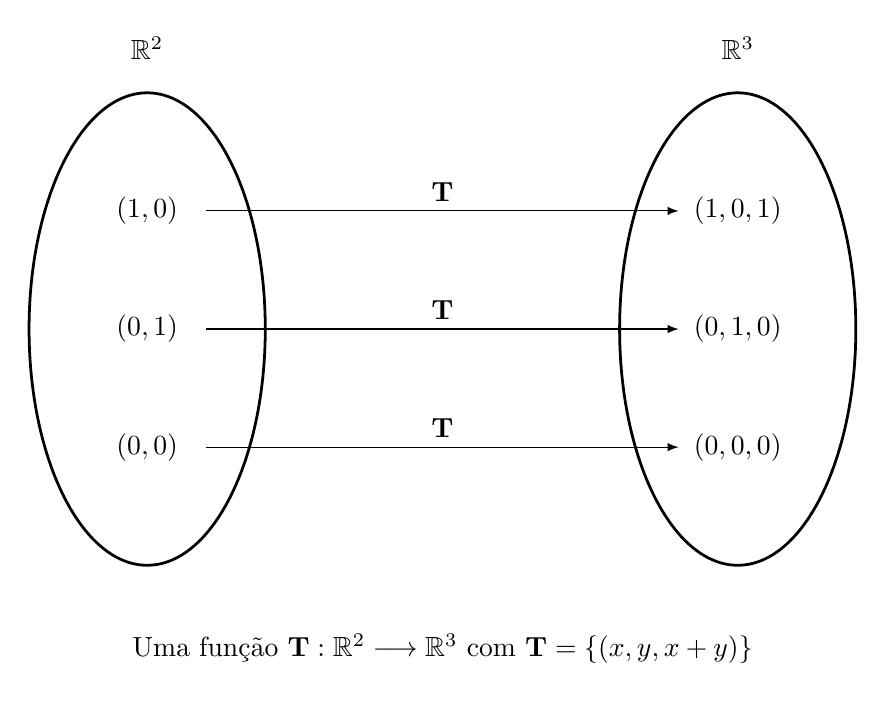
\begin{tikzpicture}[scale=1.5]
	\centering
	% Set A
	\draw[line width=1pt] (0,0) ellipse (1cm and 2cm);
	\node[above] at (0,2.2) (A) {$\mathbb{R}^2$};
	\node[centered] at (0,1) {$(1,0)$};
	\node[centered] at (0,0) {$(0,1)$};
	\node[centered] at (0,-1) {$(0,0)$};
	% Set B
	\draw[line width=1pt] (5,0) ellipse (1cm and 2cm);
	\node[above] at (5,2.2) (B) {$\mathbb{R}^3$};
	\node[centered] at (5,1) {$(1,0,1)$}; 
	\node[centered] at (5,0) {$(0,1,0)$};
	\node[centered] at (5,-1) {$(0,0,0)$};
	
	% Relations
	\draw[-latex, black] (0.5,1) -- node[midway, above] {$\mathbf{T}$} (4.5,1);
	\draw[-latex, black] (0.5, 0) -- node[midway, above] {$\mathbf{T}$} (4.5, 0);
	\draw[-latex, black] (0.5, -1) -- node[midway, above] {$\mathbf{T}$} (4.5, -1);
	
	% Label
	\node[below] at (2.5,-2.5) {Uma função $\mathbf{T}: \mathbb{R}^2 \longrightarrow \mathbb{R}^3$ com $\mathbf{T}=\{(x, y, x + y)\}$};
\end{tikzpicture}

\noindent\textbf{Exemplo 12:} Se tomarmos um vetor arbitrário e fazemos uma transformação linear idêntica, ou seja, $1\alpha$ = $\alpha$, é uma transformação linear de $\mathbf{V}$ em $\mathbf{V}$. A transformação é definida por $0\alpha = 0$, é também uma transformação linear de $\mathbf{V}$ em $\mathbf{V}$ \cite{hoffman1979}.

De acordo com o exemplo acima, percebe-se, que será uma função onde o gráfico passa a reta pela origem se supormos uma função afim, $\mathbb{R}^1$ em $\mathbb{R}^1$. Uma transformação linear mantém combinações lineares $W = [\mathbf{v}_1, \ldots, \mathbf{v}_n]$ são vetores que pertencem a $\mathbf{V}$ e possui seus escalares $c_1, \ldots, c_n$, então:

\centerline{$\mathbf{T}(c_1\mathbf{v}_1, \ldots, c_n\mathbf{v}_n) = \mathbf{T}(c_1\mathbf{v}_1 + c_2\mathbf{v}_2) = c_1(\mathbf{T}\mathbf{v}_1) + c_2(\mathbf{T}\mathbf{v}_2)$}

\noindent\textbf{Exemplo 13:} Tomemos um caso que desejamos dobrar nosso espaço vetorial, dado um vetor $\mathbf{V} = (2, 2); \mathbf{V} in \mathbb{R}^2$, a transformação linear será dada por, $\mathbf{T}(x, y) = (2x, 2y) in \mathbb{R}^2$. Nosso domínio e contradomínio está em $\mathbb{R}^2$, portanto o resultado será por $\mathbf{W} = (2 \times 2, 2 \times 2) \therefore \mathbf{W} = (4, 4)$

\begin{figure}[H]
	\centering
	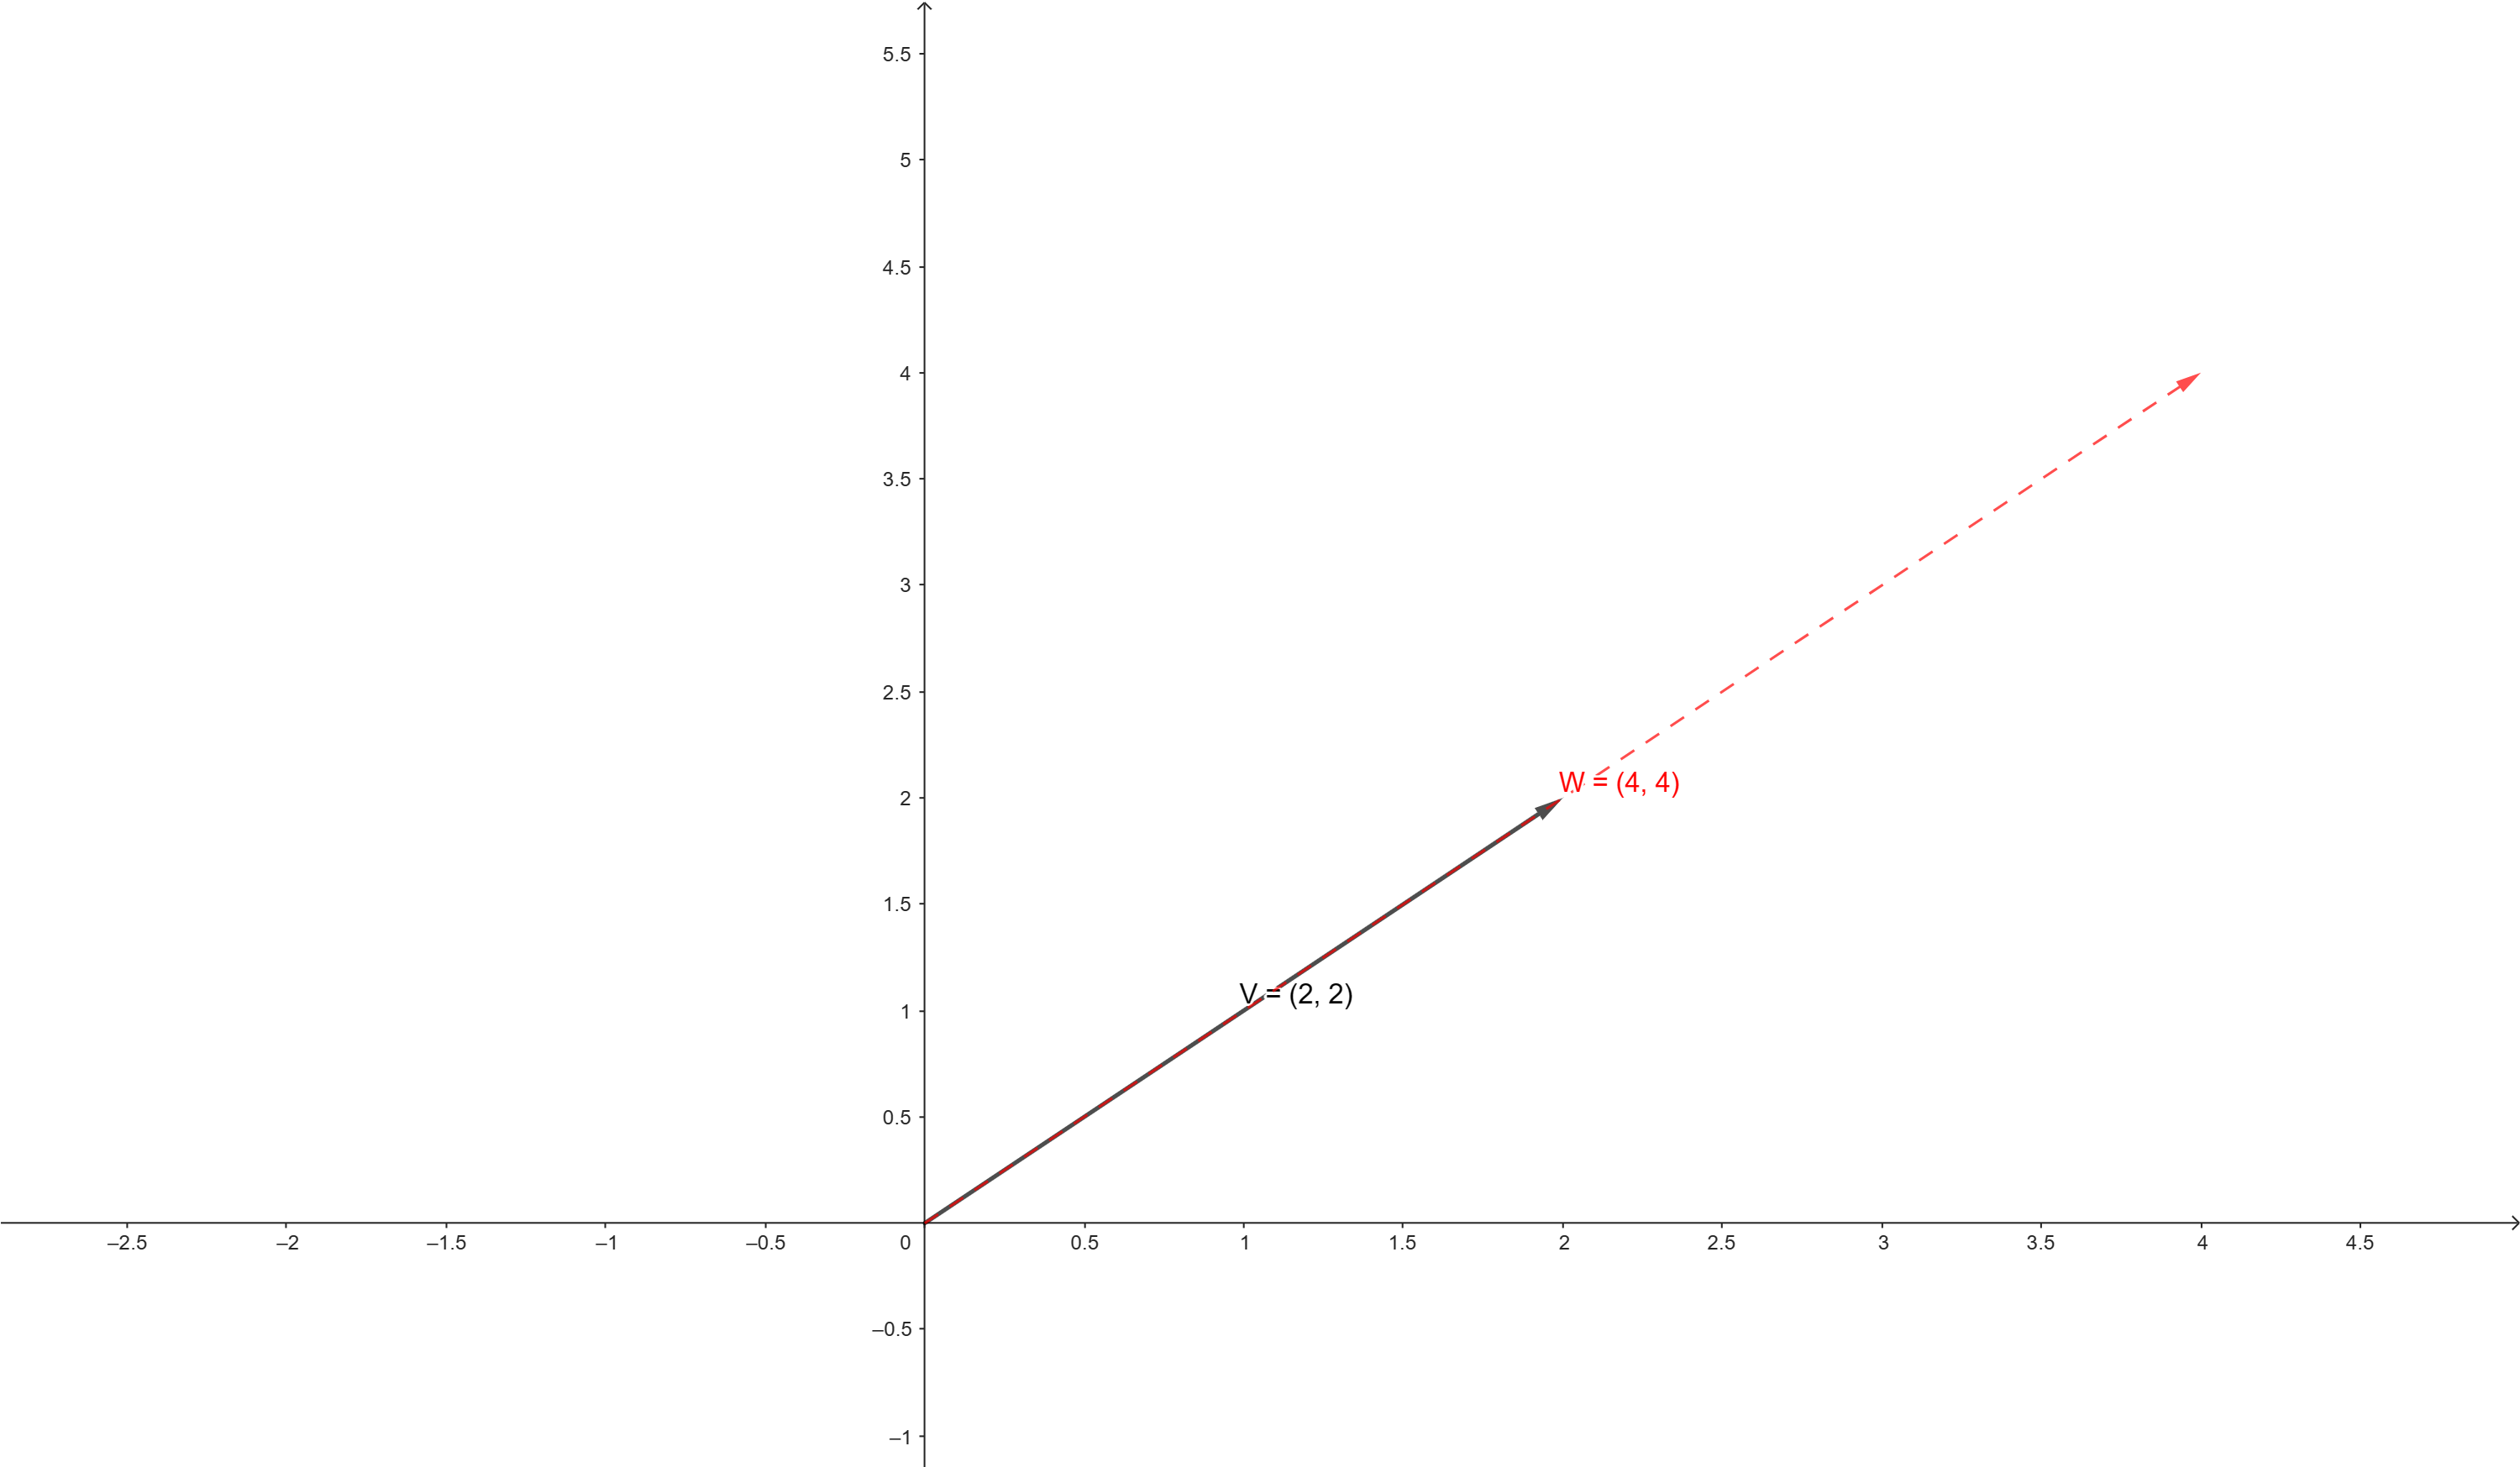
\includegraphics[scale=1.30]{t_exemplo13.png}
	\caption{Exemplo 13.}
\end{figure}

Para uma matriz de transformação linear $\mathbf{T}$ de $\mathbf{V}$ em si mesma, existe uma matriz única $\mathbf{A}$ de dimensão $ n \times n$ que representa $\mathbf{T}$. Essa matriz é definida pela seguinte propriedade:

\centerline{$\mathbf{T}(\mathbf{v} = \mathbf{A}\mathbf{v})$}

\noindent para todo vetor $\mathbf{v}$ em $\mathbf{V}$. A matriz $\mathbf{A}$ é chamada de matriz de transformação de $\mathbf{T}$.

% Primeira aplicação citada da transforamação
Consideremos agora no segmento da transformação linear e no campo da geometria o uso de operações como rotações, reflexões e projeções. Tomemos o espaço vetorial bidimensional $\mathbb{R}^2$ com base canônica $\mathbf{e}_1 = (1, 0)$ e $\mathbf{e}_2 = (0, 1)$. A rotação de 90 graus no sentido anti-horário pode ser representada pela seguinte matriz de transformação:

\centerline{$\mathbf{R} = [[0, 1], [-1, 0]]$}

A matriz $\mathbf{R}$ chamada de matriz de rotação, possui algumas propriedades:

\begin{enumerate}
	\item \textbf{Ortogonalidade:} A matriz $\mathbf{R}$ é ortogonal, ou seja sua transporta é inversa:
	
	\centerline{$\mathbf{R}^T = \mathbf{R}^{-1}$}
	\item \textbf{Determinante:} O determinante da matriz $\mathbf{R}$ é igual a $-1$.
	
	\centerline{$\det(\mathbf{R}) = -1$}
\end{enumerate}

Ao rotacionar um vetor $\mathbf{v} = (x, y)$ em 90 graus  no sentido anti-horário, basta aplicar a matriz de rotação em $\mathbf{v}$.

\centerline{$\mathbf{v}' = \mathbf{R} \times \mathbf{v} = [[-1, 0], [0, -1]] \times [x, y] = [y, -x]$}

No caso em questão, o operador de rotação de um angulo qualquer como $\theta$ em torno e origem em $\mathbb{R}^2$, tratando-se o operador $\mathbf{R}: \mathbb{R}^2 \longrightarrow \mathbb{R}^2$, resulta em $\mathbf{R}(u + v) = \mathbf{R}(u) + \mathbf{R}(v)$.

\begin{figure}[H]
	\centering
	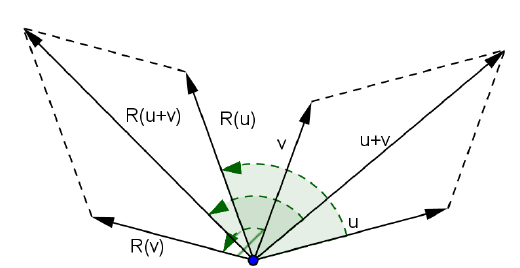
\includegraphics[scale=0.90]{t_rotacao.png}
	\caption{Retirado de \cite{nogueira2013}}
\end{figure}

\section{Núcleo de uma Transformação Linear}
Em transformações lineares. O núcleo, também chamado de espaço nulo de uma transformação linear $\mathbf{T}$, denotado por  $\mathbf{N}(\mathbf{T})$, é o conjunto de todos os vetores no domínio de $\mathbf{T}$ que são mapeados para o vetor nulo. Portanto, representa o conjunto de soluções para a equação homogênea $\mathbf{T}(x) = 0$. O núcleo é definido como:

\centerline{$\mathbf{N}(\mathbf{T}) = \{x \in \mathbf{U} \mid \mathbf{T}(x) = 0\}$}

\noindent onde $\mathbf{U}$ representa o domínio de $\mathbf{T}$.

Para $\mathbf{N}(\mathbf{T}) = \{\mathbf{v} \in \frac{\mathbf{V}}{\mathbf{T}(\mathbf{v})} = 0\}$, segue o diagrama:

\begin{figure}[H]
	\centering
	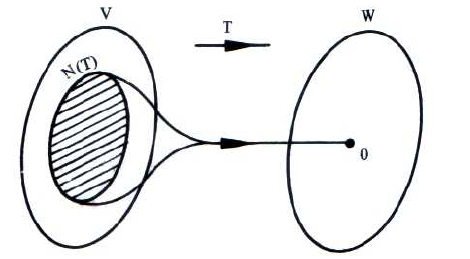
\includegraphics[scale=1.00]{t_nucleo.png}
	\caption{Retirado de \cite{steinbruch1987}}
\end{figure}

\noindent então, $\mathbf{N}(\mathbf{T}) \subset \mathbf{V}$ e $\mathbf{N}(\mathbf{T}) \neq \emptyset$, pois $0 \in \mathbf{N}(\mathbf{T})$, se $\mathbf{T}(0) = 0$.

De acordo com \cite{lang2003}, que, enfatizou a importância do núcleo na compreensão da injetividade de uma transformação linear, ou seja, a capacidade de preservar a identidade dos vetores. O núcleo de uma transformação linear possui duas propriedades, que regem:

\begin{enumerate}
	\item O núcleo de uma transformação linear $\mathbf{T}: \mathbf{V} \longrightarrow \mathbf{W}$ é um subespaço vetorial de $\mathbf{V}$.
	\item Uma transformação linear $\mathbf{T}: \mathbf{V} \longrightarrow \mathbf{W}$ é injetora se, e somente se, $\mathbf{N}(\mathbf{T}) = \{0\}$.
\end{enumerate}

Se $\mathbf{v)}_1$ e $\mathbf{v)}_2$ pertencem ao núcleo $\mathbf{N}(\mathbf{T})$ e $k$ um número real qualquer. Então, $\mathbf{T}(\mathbf{v}_1) = 0$ e $\mathbf{T}(\mathbf{v}_2) = 0$. Logo:

\centerline{$\mathbf{T}(\mathbf{v}_1 + \mathbf{v}_2) = \mathbf{T}(\mathbf{v}_1) + \mathbf{T}(\mathbf{v}_2) = 0 + 0 = 0$}

\noindent portanto, $\mathbf{v}_1 + \mathbf{v}_2 \in \mathbf{N}(\mathbf{T})$. 

\noindent\textbf{Exemplo 14:} Dado $\mathbf{T}: \mathbb{R}^2 \longrightarrow \mathbb{R} \mid (x, y) \rightarrow x + y$, o núcleo, que iremos chamar, neste caso, $\ker\mathbf{T}$ é $\ker\mathbf{T} = \{(x, y) \in \mathbb{R}^2; x + y = 0\}$, onde a reta $y = -x$ é $\ker\mathbf{T}$ e $\ker\mathbf{T} = \{(x, -x); x \in \mathbb{R}\} = \{x(1, -1); x \in \mathbb{R}\} = [(1, -1)]$. A imagem da transformação, ou seja, $Im\mathbf{T} = \mathbb{R}$, todavia, um vetor $\mathbf{w} \in \mathbb{R}, \mathbf{w} = \mathbf{T}(\mathbf{w}, 0)$.

\begin{figure}[H]
	\centering
	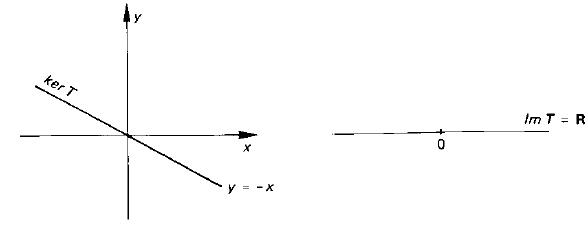
\includegraphics[scale=1.00]{t_nucleo2.png}
	\caption{Retirado de \cite{boldrini1980}, pg. 152}
\end{figure}

Percebe-se que a imagem de uma transformação é $\mathbf{T}: \mathbf{V} \longrightarrow \mathbf{W}$ é um subespaço de $\mathbf{W}$, pois, se tomarmos dois vetores, $\mathbf{w}_1 + \mathbf{w}_2 \in Im\mathbf{T}$ e $\alpha\mathbf{w}_1 \in Im\mathbf{T}$. Existem vetores $\mathbf{v}$ e $\mathbf{u} \in \mathbf{V} \mid \mathbf{T}(\mathbf{v}) = \mathbf{w}_1 + \mathbf{w}_2$ e $\mathbf{T}(\mathbf{u}) = \alpha\mathbf{w}_1$.

Se $\mathbf{w}_1, \mathbf{w}_2 \in Im\mathbf{T}$, existem vetores $\mathbf{v}_1, \mathbf{v}_2 \in \mathbf{V} \mid \mathbf{T}(\mathbf{v}_1) = \mathbf{w}_1$ e $\mathbf{T}(\mathbf{v}_2) = \mathbf{w}_2$. Tendo $\mathbf{v} = \mathbf{v}_1 + \mathbf{v}_2$ e $\mathbf{u} = \alpha\mathbf{v}_1$, logo:

\centerline{$\mathbf{T}(\mathbf{v}) = \mathbf{T}(\mathbf{v}_1 + \mathbf{v}_2) = \mathbf{T}(\mathbf{v}_1) + \mathbf{T}(\mathbf{v}_2) = \mathbf{w}_1 + \mathbf{w}_2$} 
\noindent e $\mathbf{T}(\mathbf{u}) = \mathbf{T}(\alpha\mathbf{v}_1) = \alpha\mathbf{T}(\mathbf{v}_1) = \alpha\mathbf{w}_1$, portanto, $Im\mathbf{T}$ é um subespaço vetorial de $\mathbf{W}$.

\section{Isomorfismo}
Um conceito intrigante surge com o isomorfismo. Uma transformação linear $\mathbf{T}: \mathbf{U} \longleftrightarrow \mathbf{V}$, entre espaços vetoriais $\mathbf{U}$ e $\mathbf{V}$, que é bijetora. Um isomorfismo só é válido se atender a duas condições cruciais:

\begin{enumerate}
	\item \textbf{Injetividade:} $\mathbf{T}$ é injetora, o que significa que mapeia vetores distintos do domínio para vetores distintos no contradomínio. Em outras palavras, $\mathbf{T}$ preserva a identidade.
	\item \textbf{Sobrejetividade:} $\mathbf{T}$ é sobrejetora, mapeando todo vetor em $\mathbf{V}$ a partir de um vetor em $\mathbf{U}$. Isso significa que a imagem de $\mathbf{T}$ abrange todo o espaço $\mathbf{V}$.
\end{enumerate}

\begin{figure}[H]
	\centering
	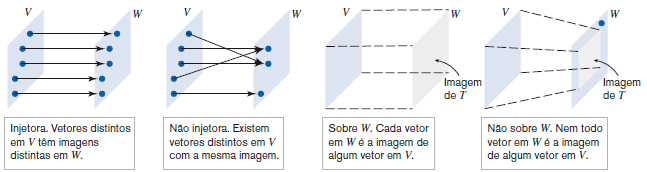
\includegraphics[scale=0.90]{t_isomorfismo.png}
	\caption{Retirado de \cite{anton2010elementary}, pg. 445}
\end{figure}

Se $\mathbf{T}$ satisfaz ambas as condições, podemos afirmar que ela estabelece uma correspondência biunívoca entre $\mathbf{U}$ e $\mathbf{V}$. Essa relação especial permite que representamos cada vetor em $\mathbf{V}$  por um único vetor em $\mathbf{U}$, e vice-versa. É notável também ressaltar, que, todo espaço vetorial $\mathbf{V}$ de dimensão $n$ é isomorfo a $\mathbb{R}^n$, portanto dois espaços vetoriais de dimensão finita são isomorfos se tiverem a mesma dimensão.

O núcleo de uma transformação e seu isomorfismo tem uma conexão que é o Teorema do Núcleo e da Imagem. Este teorema estabelece uma relação crucial entre a dimensão do núcleo, a dimensão da imagem e a dimensão do domínio de uma transformação linear $\mathbf{T}$:

\centerline{$\dim(\mathbf{N}(\mathbf{T})) + \dim(Im(\mathbf{T})) = \dim(\mathbf{U})$}

\noindent onde $Im(\mathbf{T})$ representa a imagem de $Im(\mathbf{T})$, o conjunto de todos os vetores em $\mathbf{V}$ que são alcançados por $\mathbf{T}$.

O Teorema do Núcleo e da Imagem oferece ferramentas valiosas para determinar se uma transformação linear é um isomorfismo. Se a dimensão do núcleo for zero e a dimensão da imagem for igual à dimensão do domínio, podemos concluir que $\mathbf{T}$ é um isomorfismo.

\noindent\textbf{Teorema:} Sejam $E, F$ espaços vetoriais de dimensão finita. Para toda transformação linear $\mathbf{T}: E \longrightarrow F$ tem-se que $\dim E = \dim \mathbf{N}(\mathbf{T}) + \dim Im(\mathbf{T})$.

Se $\{\mathbf{T}(\mathbf{u}_1), \ldots, \mathbf{T}(\mathbf{u}_p)\}$ é uma base de $Im(\mathbf{T})$ e $\{\mathbf{v}_1, \ldots, \mathbf{v}_q\}$ é uma base de $\mathbf{N}(\mathbf{T})$ então $\{\mathbf{u}_1, \ldots, \mathbf{u}_p, \mathbf{v}_1, \ldots, \mathbf{v}_q\}$ é uma base de $E$. Logo, se tivemos

\centerline{$\alpha_1\mathbf{u}_1 + \ldots + \alpha_p + \beta\mathbf{v}_1 + \ldots + \beta\mathbf{u}_q = 0$,}

então, com a transformação em ambos os membros da igualdade, obtemos

\centerline{$\alpha_1\mathbf{T}(\mathbf{u}_1) + \ldots + \alpha_p\mathbf{T}(\mathbf{u}_p) = 0$.}

Como $\mathbf{T}(\mathbf{u}_1), \ldots, \mathbf{T}(\mathbf{u}_p)$ são \textbf{LI}, resultando em $\alpha_1 = \ldots = \alpha_p = 0$. Portanto se reduz a igualdade

\centerline{$\beta_1\mathbf{v}_1 + \ldots + \beta_q\mathbf{v}_q = 0$.}

Da mesma forma $\mathbf{v}_1, \ldots, \mathbf{v}_q$ são \textbf{LI}, concluí-se que $\beta_1 = \ldots = \beta_q = 0$. Então ambos os vetores $\mathbf{u}$ e $\mathbf{v}$ são \textbf{LI}.

Agora, se considerarmos um vetor arbitrário $\mathbf{w} \in E$. Como $\mathbf{T}(\mathbf{w}) \in Im(\mathbf{T})$, definimos

\centerline{$\mathbf{T}(\mathbf{w}) = \alpha_1\mathbf{T}(\mathbf{u}_1) + \ldots + \alpha_p\mathbf{T}(\mathbf{u}_p)$,}

pois $\{\mathbf{T}(\mathbf{u}_1), \ldots, \mathbf{T}(\mathbf{u}_p)\}$ é uma base da imagem de $\mathbf{T}$. Manipulando a expressão temos

\centerline{$\mathbf{T}[\mathbf{w} - (\alpha_1\mathbf{u}_1 + \ldots + \alpha_p\mathbf{u}_p)] = 0$.}

Dessa forma, o vetor $\mathbf{w} - (\alpha_1\mathbf{u}_1 + \ldots + \alpha_p\mathbf{u}_p)$ pertence ao núcleo de $\mathbf{T}$, podendo ser expresso como uma combinação linear dos elementos da base $\{\mathbf{v}_1, \ldots, \mathbf{v}_q\}$. Temos então

\centerline{$(\alpha_1\mathbf{u}_1 + \ldots + \alpha_p\mathbf{u}_p) = \beta_1\mathbf{v}_1 + \ldots + \beta_q\mathbf{v}_q$,}

ou seja, $\mathbf{w} = \alpha_1\mathbf{u}_1 + \ldots + \alpha_p\mathbf{u}_p + \beta_1\mathbf{v}_1 + \ldots + \beta_q\mathbf{v}_q$. O que prova que os vetores $\{\mathbf{u}_1, \ldots, \mathbf{u}_p, \mathbf{v}_1, \ldots, \mathbf{v}_q\}$ geram $E$ e portanto constituem uma base.

	
	\chapter{Aplicações de Transformações Lineares}
As TL têm contribuições significativas para o campo da AL. \cite{strang2010}, renomado matemático e professor do MIT - Massachusetts Institute of Technology, aborda, por exemplo, o processamento de sinais e imagens para compressão, filtragem, reconstrução e análise de dados, a análise de redes e sistemas dinâmicos da engenharia elétrica e ciência da computação, a geometria e a computação gráfica para manipular objetos em espaços tridimensionais, videogames e modelagem em três dimensões, além de cripto segurança e, mais recentemente, análise de dados em decisões gerenciais e aprendizagem de máquina. \nocite{pitombeira1971}

A seguir, baseando em um estudo desenvolvido na Universidade Federal de Alagoas \cite{sirlandro2017}, apresentamos algumas aplicações das TL na área de engenharia.

\section{Circuitos Elétricos}
Um circuito elétrico é composto por geradores que criam correntes elétricas com magnitudes limitadas pelos resistores posicionados em série ou em paralelo, exemplificado na figura 12. Existem três unidades básicas da física: potencial elétrico $\mathbf{V}$(volts = $\mathbf{V}$), resistência elétrica $\mathbf{R}$(ohms = $\Omega$) e corrente elétrica $\mathbf{I}$(ampères = $\mathbf{A}$), como por exemplo, baterias, que mantêm a diferença de potencial constante entre seus dois terminais.

\begin{figure}[H]
	\centering
	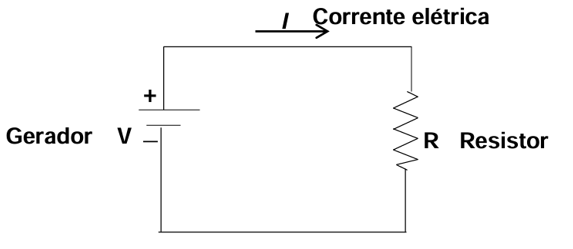
\includegraphics[scale=0.90]{a_fg1.png}
	\caption{Diagrama de circuito elétrico \cite{sirlandro2017}.}
\end{figure}

Para a montagem ou avaliação de um circuito, é necessário descobrir qual a corrente elétrica que passa em cada trecho do circuito e as quedas de potencial. Dependendo do fluxo da corrente elétrica, as intensidades de corrente e as quedas de tensão podem ser positivas ou negativas. Três princípios básicos devem ser considerados:

\begin{itemize}
	\item \textbf{Lei de Ohm:} A diferença de potencial medida através de um resistor é o produto da corrente que passa por ele e a sua resistência, representado por
	
	\centerline{$\mathbf{V} = \mathbf{R} \times \mathbf{I}$},
	onde $\mathbf{V}$ é a tensão, em Volts($\mathbf{V}$, $\mathbf{R}$ é a resistência, em ohm($\Omega$) e $\mathbf{I}$ é a corrente, em ampère($\mathbf{A}$).
	
	\item \textbf{Lei da corrente de Kirchhoff:} Se houver um ponto de ramificação, junção ou nó, a corrente pode se dividir e a soma das correntes que chegam no nó devem ser iguais à soma das correntes que saem do nó, representado por
	
	\centerline{$\mathbf{I} = \mathbf{I}_1 + \mathbf{I}_2$}
	
	\item \textbf{Lei das malhas ou Lei de Voltagem de Kirchhoff:} A soma algébrica das variações no potencial ao longo de qualquer malha fechada deve ser igual a zero. Para exemplificar a aplicação das leis, considera-se o circuito da figura
	
	\begin{figure}[H]
		\centering
		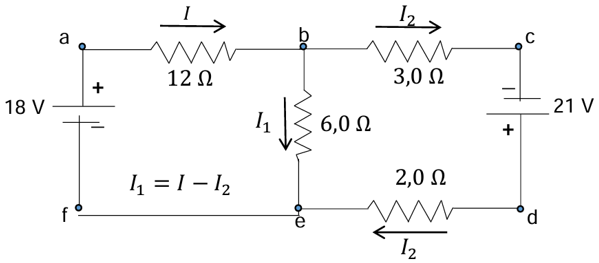
\includegraphics[scale=0.90]{a_fg2.png}
		\caption{Circuito de malha de resistência elétrica \cite{sirlandro2017}.}
	\end{figure}
\end{itemize}

Considerando a lei dos nós no trecho $\overrightarrow{abefa}$, obtemos a equação

\centerline{$18\mathbf{V} - (12\Omega)\mathbf{I} - (6\Omega)\mathbf{I}_1 = 0$}

Aplicando a lei das malhas no trecho $\overrightarrow{abefa}$, obtemos a equação

\centerline{$-(3\Omega)\mathbf{I}_2 + 21\mathbf{V} - (2\Omega)\mathbf{I}_2 + (6\Omega)\mathbf{I}_1 = 0$}

Para determinar as correntes, resolvemos o sistema de equações lineares

\begin{enumerate}
	\item $\mathbf{I} = \mathbf{I}_1 + \mathbf{I}_2$
	\item $18 - 12\mathbf{I} - 6\mathbf{I}_2 = 0$
	\item $21 - 5\mathbf{I}_2 + 6\mathbf{I}_1 = 0$
\end{enumerate}

Dividimos a equação 2 por 6:

\begin{enumerate}
	\item $\mathbf{I} = \mathbf{I}_1 + \mathbf{I}_2$
	\item $3 - 2\mathbf{I} - \mathbf{I}_1 = 0$
	\item $21 - 5\mathbf{I}_2 + 6\mathbf{I}_1 = 0$
\end{enumerate}

Representado em matriz aumentada, temos o sistema consistente

\[
\left[
\begin{array}{ccc|c}
	1 & -1 & -1 & 0\\
	-2 & -1 & 0 & -3\\
	0 & 6 & -5 & 21\\
\end{array}
\right]
\]

Utilizando o método de Gauss-Jordan, podemos adotar a seguinte sequência:
\begin{enumerate}
 
	\item Multiplicar a primeira linha por 2:
	\[
	\begin{bmatrix}
		2 & -2 & -2 & 0 \\
		-2 & -1 & 0 & -3 \\
		0 & 6 & -5 & 21 \\
	\end{bmatrix}
	\]
	
	\item Somar o resultado à linha 2:
	\[
	\begin{bmatrix}
		2 & -2 & -2 & 0 \\
		0 & -3 & -2 & -3 \\
		0 & 6 & -5 & 21 \\
	\end{bmatrix}
	\]
	
	\item Multiplicar a linha 2 por 2:
	\[
	\begin{bmatrix}
		2 & -2 & -2 & 0 \\
		0 & -6 & -4 & -6 \\
		0 & 6 & -5 & 21 \\
	\end{bmatrix}
	\]
	
	\item Somar o resultado à linha 3:
	\[
	\begin{bmatrix}
		2 & -2 & -2 & 0 \\
		0 & -6 & -4 & -6 \\
		0 & 0 & -9 & 15 \\
	\end{bmatrix}
	\]
	
	\item Multiplicar a linha 3 por $-\frac{1}{9}$:
	\[
	\begin{bmatrix}
		2 & -2 & -2 & 0 \\
		0 & -6 & -4 & -6 \\
		0 & 0 & 1 & -\frac{5}{3} \\
	\end{bmatrix}
	\]
	
	\item Multiplicar a linha 3 por 1:
	\[
	\begin{bmatrix}
		2 & -2 & -2 & 0 \\
		0 & -6 & -4 & -6 \\
		0 & 0 & 1 & -\frac{5}{3} \\
	\end{bmatrix}
	\]
	
	\item Somar à linha 1:
	\[
	\begin{bmatrix}
		2 & -2 & -1 & -\frac{5}{3} \\
		0 & -6 & -4 & -6 \\
		0 & 0 & 1 & -\frac{5}{3} \\
	\end{bmatrix}
	\]
	
	\item Multiplicar a linha 3 por 2:
	\[
	\begin{bmatrix}
		2 & -2 & -1 & -\frac{5}{3} \\
		0 & -6 & -4 & -6 \\
		0 & 0 & 2 & -\frac{10}{3} \\
	\end{bmatrix}
	\]
	
	\item Somar à linha 2:
	\[
	\begin{bmatrix}
		2 & -2 & -1 & -\frac{5}{3} \\
		0 & -6 & -2 & -\frac{28}{3} \\
		0 & 0 & 2 & -\frac{10}{3} \\
	\end{bmatrix}
	\]
	
	\item Multiplicar a linha 2 por $-\frac{1}{3}$:
	\[
	\begin{bmatrix}
		2 & -2 & -1 & -\frac{5}{3} \\
		0 & 2 & \frac{2}{3} & \frac{28}{9} \\
		0 & 0 & 2 & -\frac{10}{3} \\
	\end{bmatrix}
	\]
	
	\item Somar à linha 1:
	\[
	\begin{bmatrix}
		2 & 0 & -\frac{2}{3} & \frac{13}{9} \\
		0 & 2 & \frac{2}{3} & \frac{28}{9} \\
		0 & 0 & 2 & -\frac{10}{3} \\
	\end{bmatrix}
	\]
\end{enumerate}

Iara, os passos dão errado para o resultado final...

 

	
	% Conclusão
	\chapter{Conclusão}
That's all folks!
Teste citação: De acordo com \cite{einstein1905}, a teoria da relatividade restrita foi publicada por Einstein em 1905.

		
	% Referências Bibliográficas
	\bibliographystyle{abntex2-alf}
	\bibliography{references.bib}

		
\end{document}